\documentclass{article}

\title{Religious Coping in Times of Crisis: Evidence from COVID-19 Lockdowns and Google Trends Data}
\author{Alberto Trelles}
\date{\monthname[\month] \the\year}

    \usepackage{graphicx} % For scalebox
    \usepackage{ragged2e} % For justifying
    \usepackage{array}    % For advanced table formatting
    \usepackage{geometry} % Set margins
    \usepackage{amssymb}  % For cross and checks 
    \usepackage{pdflscape}
    \usepackage{xcolor}   % For red text
    \usepackage{booktabs} % For cmidrule
    \usepackage{multirow}
    \usepackage{multicol}
    \usepackage{dsfont}
    \usepackage{comment}
    \usepackage{amsmath}
    \usepackage{datetime}
    \usepackage{tikz}
    \usetikzlibrary{arrows.meta, decorations.pathreplacing}

    \usepackage{natbib}

    
 %For spanish language


\begin{document}
\newgeometry{left=2.5cm, right=2.5cm, top=2.5cm, bottom=2.5cm}


\section{Tables}

%--- TWFE & BJS ---%
%------------------%
\begin{table}[htb!]
\caption{DiD estimates on Topics}
\begin{center}
\scalebox{0.8}{
\def\arraystretch{1.1}
\begin{tabular}{
>{\raggedright\arraybackslash}p{4cm}
*{6}{>{\centering\arraybackslash}p{2.5cm}}
}
~ & Faith & God & Meditation & Prayer & Religion & Spirituality \\
~ & (1) & (2) & (3) & (4) & (5) & (6) \\
\hline \hline \\ [-1ex]

\multicolumn{7}{l}{\textit{I. TWFE Estimates}} \\ [2ex]
\input{../Tables/us_twfe1} \\ [0ex]

\multicolumn{7}{l}{\textit{II. BJS Estimates}} \\ [2ex]
ATT $(\tau)$        &      15.708***&      10.858***&      10.176***&      19.748***&       2.277** &      -2.750***\\
                    &     (0.781)   &     (0.397)   &     (0.514)   &     (0.695)   &     (0.996)   &     (0.792)   \\
\\
p-value             &       0.000   &       0.000   &       0.000   &       0.000   &       0.022   &       0.001   \\
Observations in $\Omega_0$&       5,829   &       7,720   &       6,572   &       7,475   &       7,457   &       6,123   \\
Observations in $\Omega_1$&         534   &         668   &         608   &         656   &         660   &         550   \\
 \\ [-2ex]

\hline \hline 

\end{tabular}
}
\end{center}
\label{tab:twfe_bjs1}
\justifying
{\scriptsize \textbf{Notes:} This table reports TWFE (Panel I) and BJS (Panel II) estimates for Google Trends topics. State, year, day-of-year and dow fixed effects are included as specified in equation \ref{eq:twfe}. Clustered standard errors at the day level in parenthesis.  *signifcantant 10\%, **signicantat 5\%,***signicantant 1\%  \par}
\end{table}



%--- 1-week anticipation ---%
%---------------------------%
\begin{table}[htb!]
\caption{DiD estimates on Topics (1-week anticipation)}
\begin{center}
\scalebox{0.8}{
\def\arraystretch{1.1}
\begin{tabular}{
>{\raggedright\arraybackslash}p{4cm}
*{6}{>{\centering\arraybackslash}p{2.5cm}}
}
~ & Faith & God & Meditation & Prayer & Religion & Spirituality \\
~ & (1) & (2) & (3) & (4) & (5) & (6) \\
\hline \hline \\ [-1ex]

\multicolumn{7}{l}{\textit{I. TWFE Estimates}} \\ [2ex]
ATT $(\gamma)$      &      12.629***&       9.142***&       6.738***&      18.258***&      -4.782***&      -5.653***\\
                    &     (1.134)   &     (0.753)   &     (1.417)   &     (1.142)   &     (1.700)   &     (1.244)   \\
\\
Mean: pre-lockdown  &       43.90   &       63.33   &       45.90   &       48.98   &       54.82   &       48.13   \\
p-value             &       0.000   &       0.000   &       0.000   &       0.000   &       0.006   &       0.000   \\
Observations        &       6,363   &       8,388   &       7,180   &       8,131   &       8,117   &       6,673   \\
 \\ [0ex]

\multicolumn{7}{l}{\textit{II. BJS Estimates}} \\ [2ex]
ATT $(\tau)$        &      14.574***&       9.949***&       7.231***&      19.221***&      -3.716***&      -5.755***\\
                    &     (0.735)   &     (0.274)   &     (0.458)   &     (0.465)   &     (0.799)   &     (0.739)   \\
\\
p-value             &       0.000   &       0.000   &       0.000   &       0.000   &       0.000   &       0.000   \\
Observations in $\Omega_0$&       5,602   &       7,426   &       6,305   &       7,188   &       7,179   &       5,894   \\
Observations in $\Omega_1$&         761   &         962   &         875   &         943   &         938   &         779   \\
 \\ [-2ex]

\hline \hline 

\end{tabular}
}
\end{center}
\label{tab:twfe_bjs2}
\justifying
{\scriptsize \textbf{Notes:} This table reports TWFE (Panel I) and BJS (Panel II) estimates for Google Trends topics. Treatment is redefined to start 7 days before announcement. State, year, day-of-year and dow fixed effects are included as specified in equation \ref{eq:twfe}. Clustered standard errors at the day level in parenthesis.  *signifcantant 10\%, **signicantat 5\%,***signicantant 1\%  \par} 
\end{table}

%--- HTE by Baseline Religiosity ---%
%------------------------------------%
\begin{table}[htb!]
\caption{Heterogeneous Effects by Baseline Religiosity Level}
\begin{center}
\scalebox{0.8}{
\def\arraystretch{1.1}
\begin{tabular}{
>{\raggedright\arraybackslash}p{4cm}
*{3}{>{\centering\arraybackslash}p{2.5cm}}
}
~ & God & Prayer & Meditation \\
~ & (1) & (2) & (3) \\
\hline \hline \\ [-1ex]

ATT $(\gamma)$      &      10.762***&      19.151***&      10.068***\\
                    &     (0.619)   &     (1.361)   &     (1.596)   \\
ATT $(\gamma_H - \gamma_L)$&      -2.611***&      -3.267***&      -2.214   \\
                    &     (0.928)   &     (0.785)   &     (1.962)   \\
\\
Mean: pre-lockdown  &       63.54   &       49.55   &       45.83   \\
p-value: ATT        &       0.000   &       0.000   &       0.000   \\
p-value: Interaction&       0.006   &       0.000   &       0.262   \\
Observations        &       8,388   &       8,131   &       7,180   \\
 \\ [-2ex]

\hline \hline

\end{tabular}
}
\end{center}
\label{tab:het1}
\justifying
{\scriptsize \textbf{Notes:} This table reports TWFE triple-DiD estimates of the heterogeneous effect of lockdown announcements by baseline religiosity level. High-religion states are defined as those above the median share of ``very religious'' adults in the Gallup 2017 U.S. Daily tracking survey. $\gamma$ captures the ATT for low-religion states; $\gamma_H - \gamma_L$ captures the differential ATT for high-religion states. State, year, day-of-year and day-of-week fixed effects included. Clustered standard errors at the day level in parentheses. *significant at 10\%, **significant at 5\%, ***significant at 1\%.  \par}
\end{table}

\newpage

\section{Figures}

%--- Timeline ---%
%----------------%
\begin{figure}[htbp]
    \centering
    \caption{Sample selection and timeline} 
    \vspace{1em}
    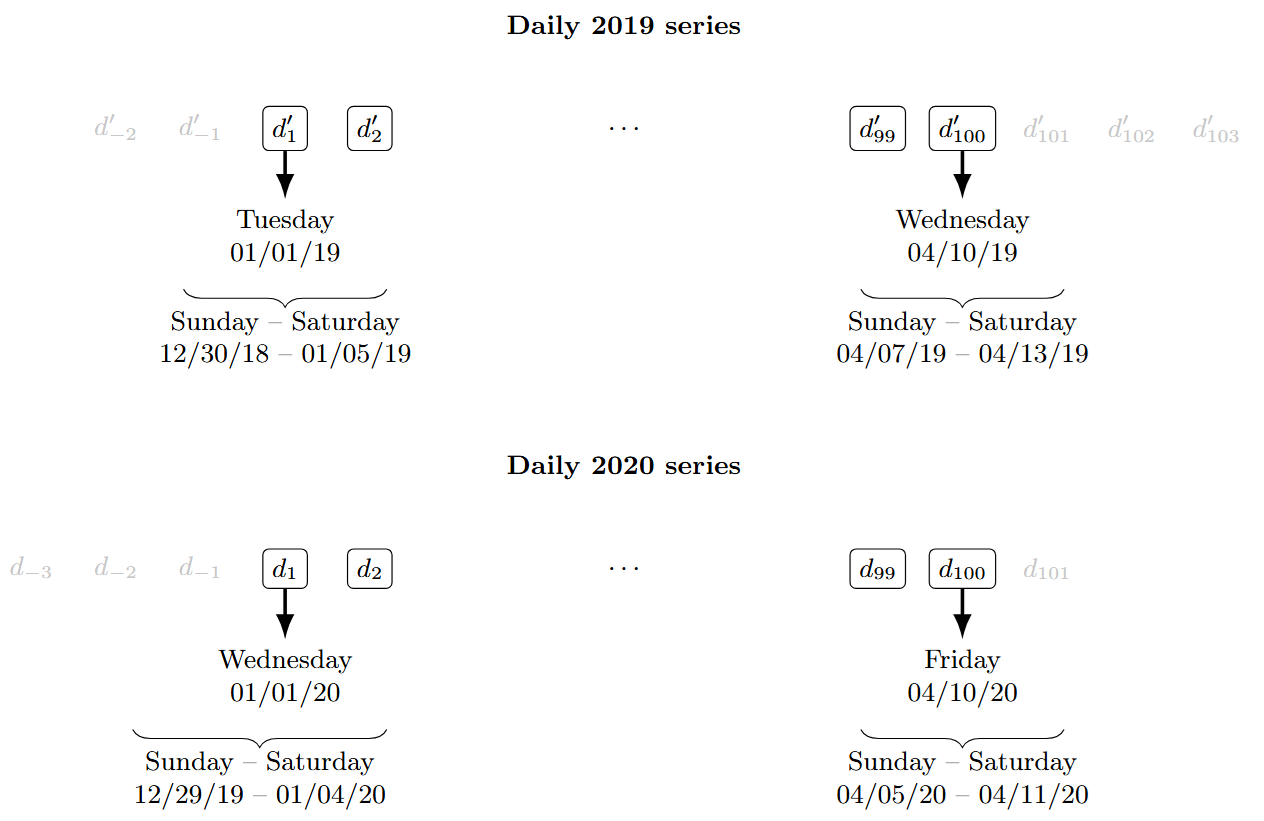
\includegraphics[width=0.9\textwidth]{../Figures/timeline.png}
    \label{fig:timeline}
\justifying \\ [3ex]    
{\scriptsize \textbf{Notes:} This figure shows the exact dates considered for analysis and rescaling process, for both 2019 and 2020 timelines. Days that are not included for regression analysis but are necessary for a proper weekly normalization process are displayed in gray.  \par}
\end{figure}

\newpage 

%--- Topics Evolution ---%
%------------------------%
\begin{figure}[htb!]
\caption{Topic Series: 2019 vs. 2020}
\centering
\begin{tabular}{cc}
\\ 

% Row 1
Faith & God \\
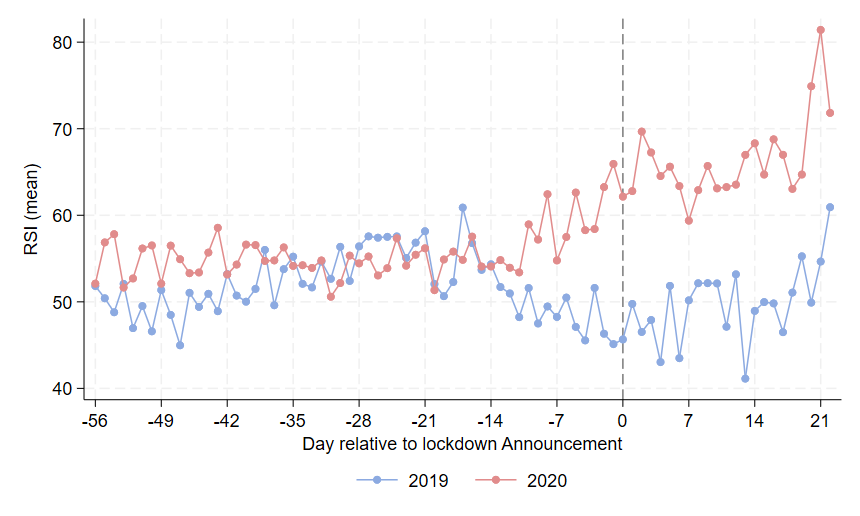
\includegraphics[scale=0.25]{../Figures/us_evolution1_Faith.png} &
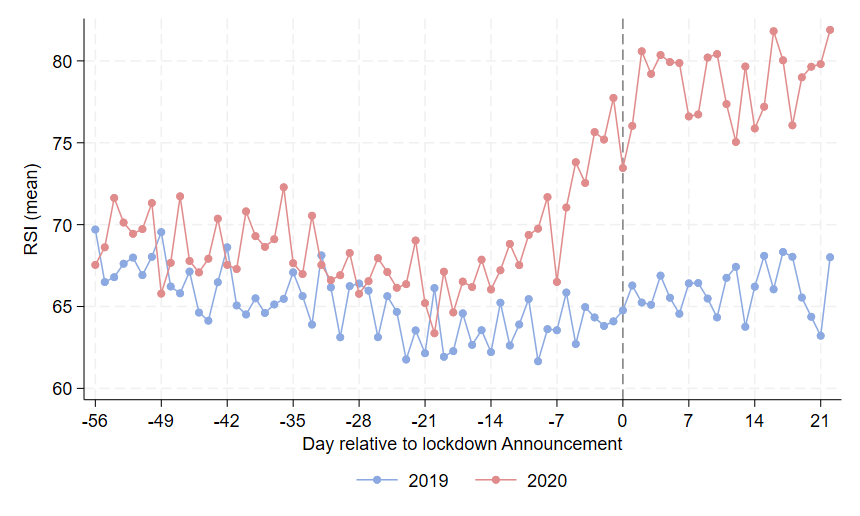
\includegraphics[scale=0.25]{../Figures/us_evolution1_God.png} \\


% Row 2
Meditation & Prayer \\
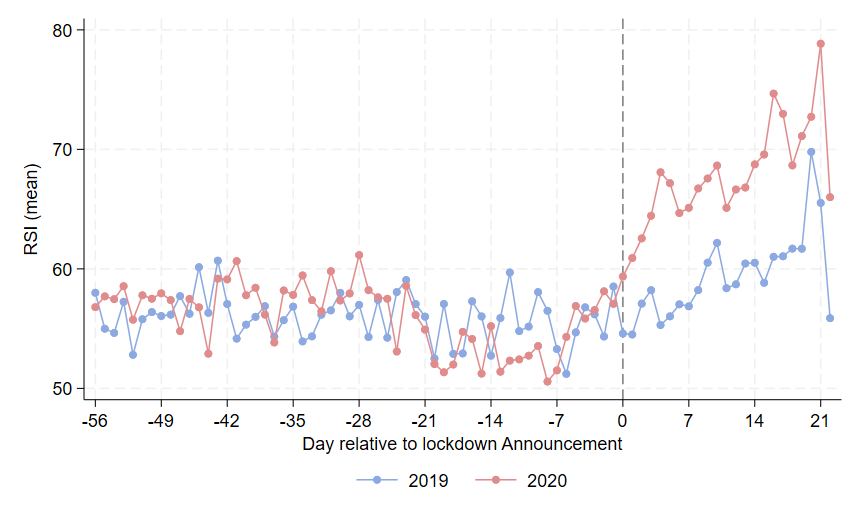
\includegraphics[scale=0.25]{../Figures/us_evolution1_Meditation.png} &
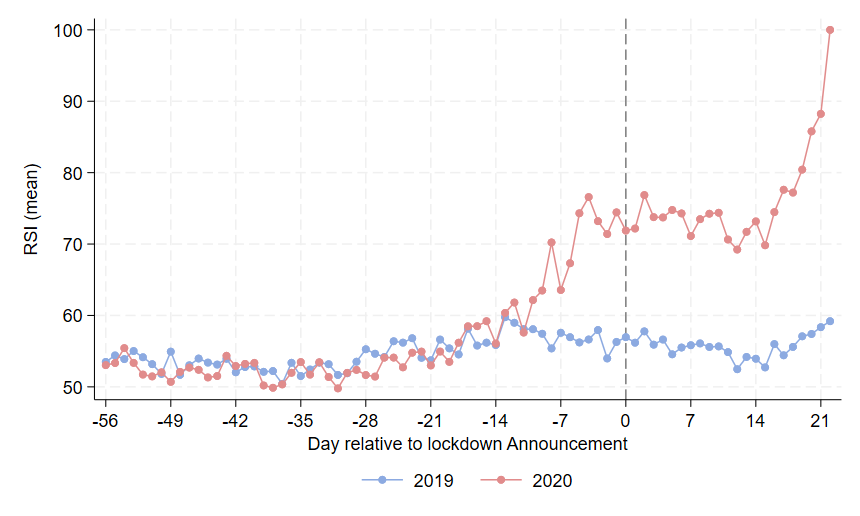
\includegraphics[scale=0.25]{../Figures/us_evolution1_Prayer.png} \\


% Row 3
Religion & Spirituality \\
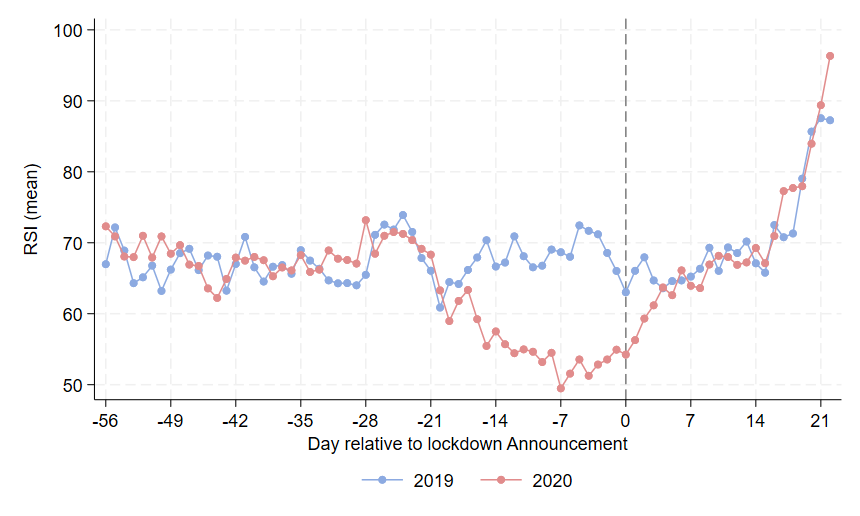
\includegraphics[scale=0.25]{../Figures/us_evolution1_Religion.png} &
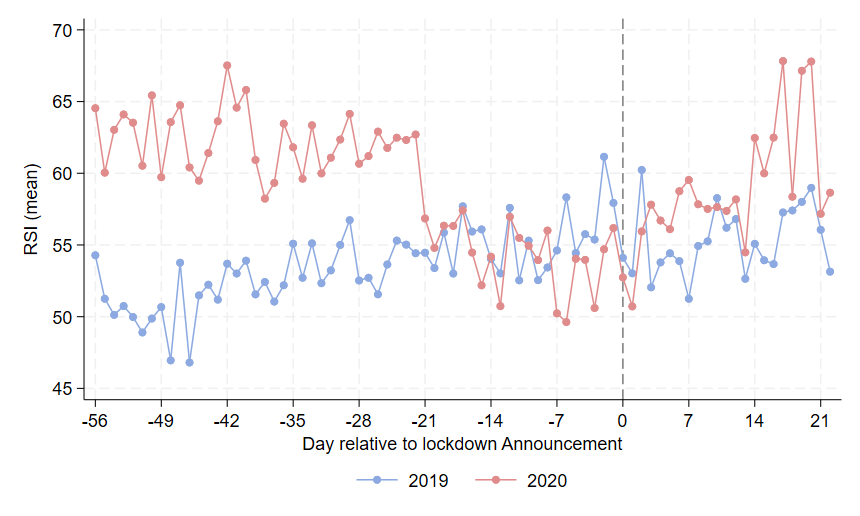
\includegraphics[scale=0.25]{../Figures/us_evolution1_Spirituality.png} \\

\label{fig:topics-evolution}
\end{tabular}
\justifying \\ [-3ex]
{\scriptsize \textbf{Notes:} This figure shows the evolution for each topic using the rescaled series for 2019 (blue) and 2020 (red). Relative days to lockdown announcement are in the x-axis. For 2019 these correspond to the paired days.  \par}
\end{figure}

\newpage

%--- Covid controls ---%
%----------------------%
\begin{figure}[htbp]
    \centering
    \caption{TWFE estimates and Covid-19 controls}
    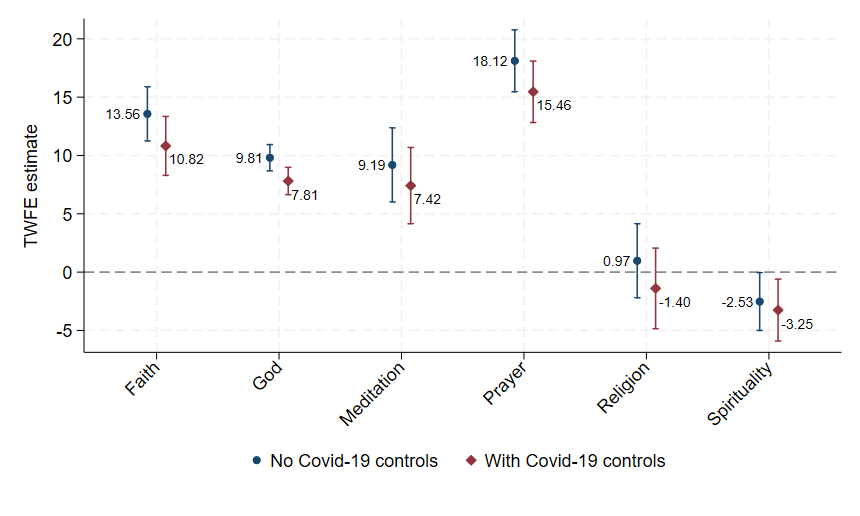
\includegraphics[width=0.9\textwidth]{../Figures/covid_controls.png}
    \label{fig:covid_controls}
\justifying \\ [-3ex]
{\scriptsize \textbf{Notes:} This figure compares TWFE estimates as in Equation \ref{eq:twfe} both including and not including one day lagged number of confirmed COVID-19 deaths. Confidence intervals at the 95\% level.  \par}
\end{figure}

\newpage 

%--- Pretrends test: Topics ---%
%------------------------------%
\begin{figure}[htb!]
\caption{Pretrends test: Topics}
\centering
\begin{tabular}{cc}
\\ 

% Row 1
Faith & God \\
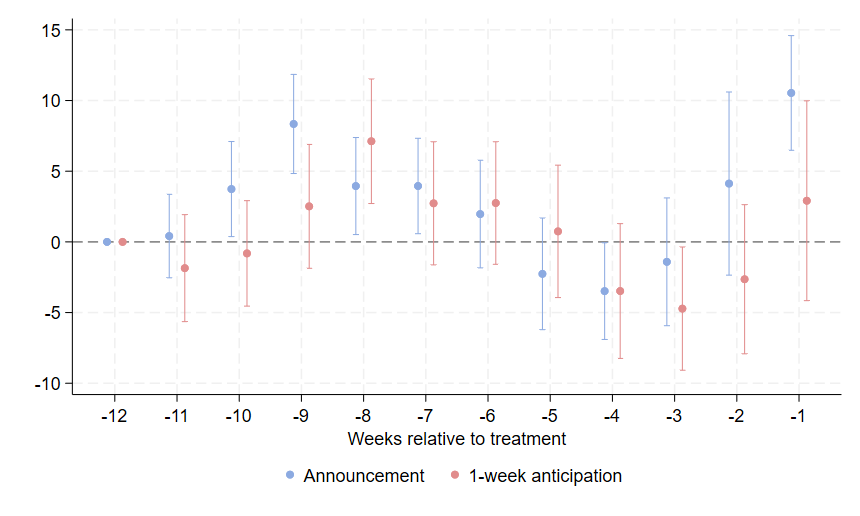
\includegraphics[scale=0.275]{../Figures/pretrends_Faith.png} &
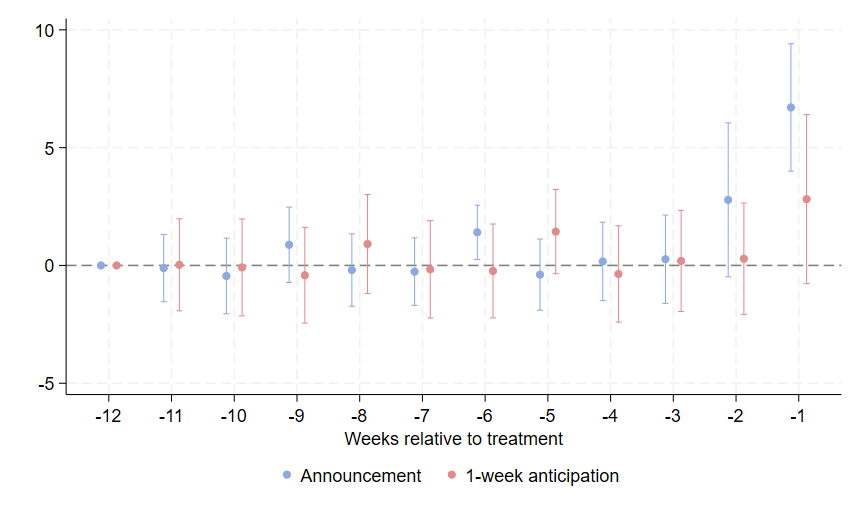
\includegraphics[scale=0.275]{../Figures/pretrends_God.png} \\


% Row 2
Meditation & Prayer \\
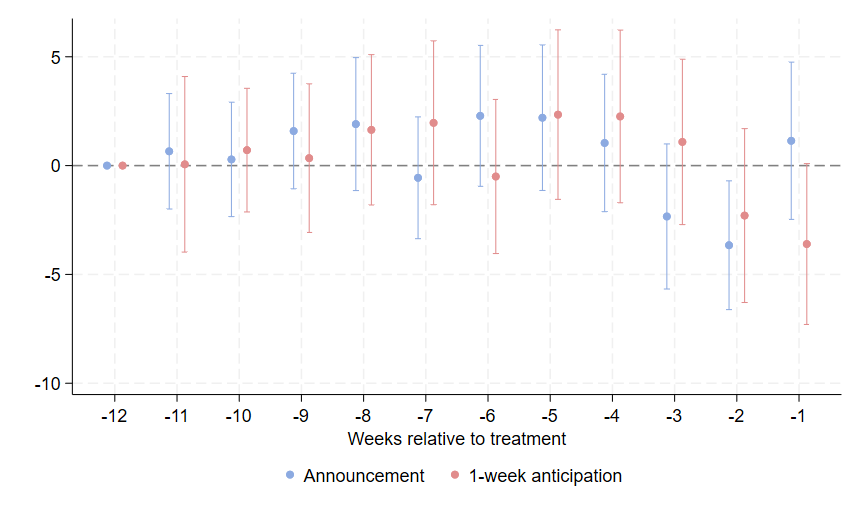
\includegraphics[scale=0.275]{../Figures/pretrends_Meditation.png} &
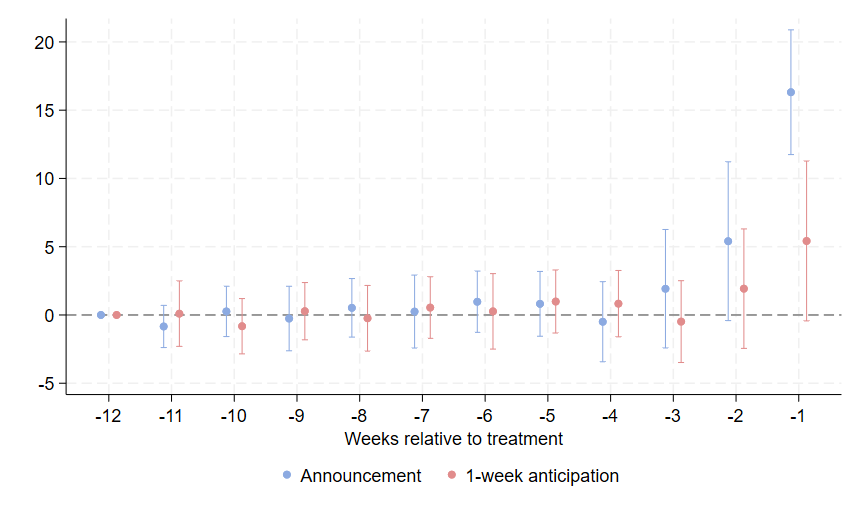
\includegraphics[scale=0.275]{../Figures/pretrends_Prayer.png} \\


% Row 3
Religion & Spirituality \\
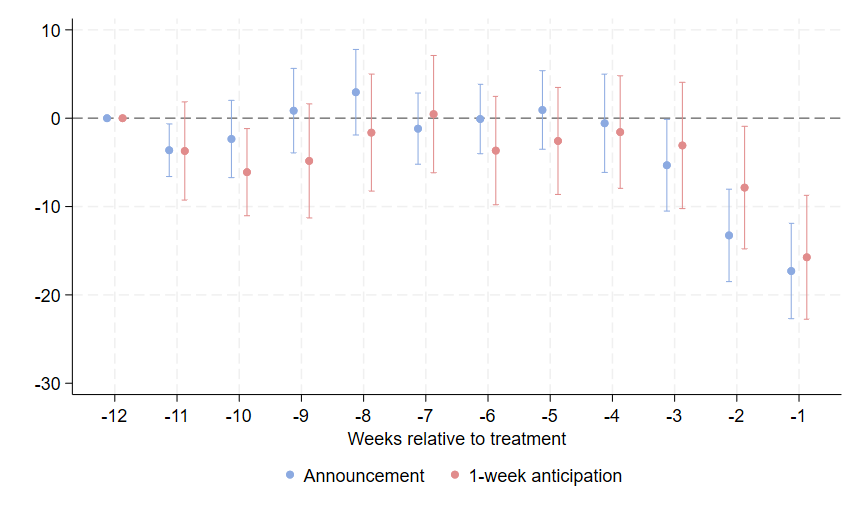
\includegraphics[scale=0.275]{../Figures/pretrends_Religion.png} &
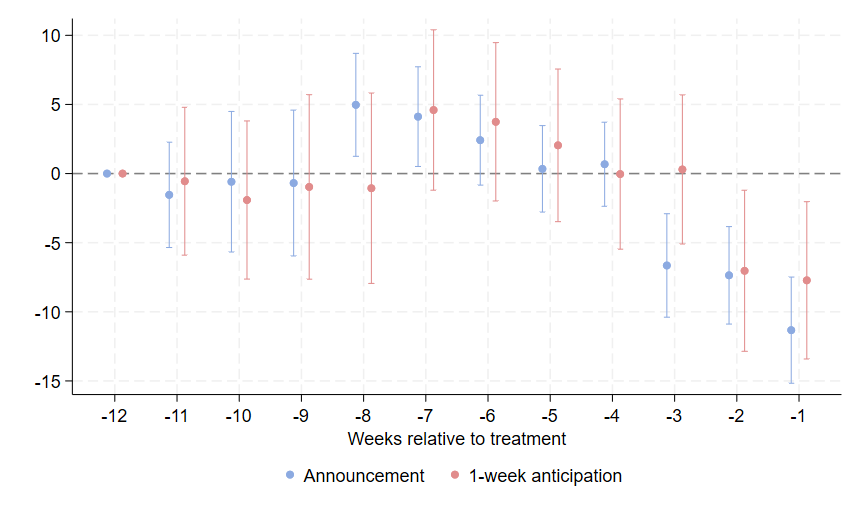
\includegraphics[scale=0.275]{../Figures/pretrends_Spirituality.png} \\

\label{fig:pre-trends}


\end{tabular}
\justifying \\ [-3ex]
{\scriptsize \textbf{Notes:} This figure reports the pre-trends test coefficients as in \ref{eq:pre-trends}. Blue lines use the lockdown announcement day as beginning of treatment, whereas as red lines redifine treatment to begin 7 days before announcement. Confidence intervals at the 95\% level. \par}
\end{figure}

\newpage

%--- Event Study HTE by Religiosity ---%
%--------------------------------------%
\begin{figure}[htb!]
\caption{Event Study by Baseline Religiosity Level}
\centering
\begin{tabular}{c}
God \\
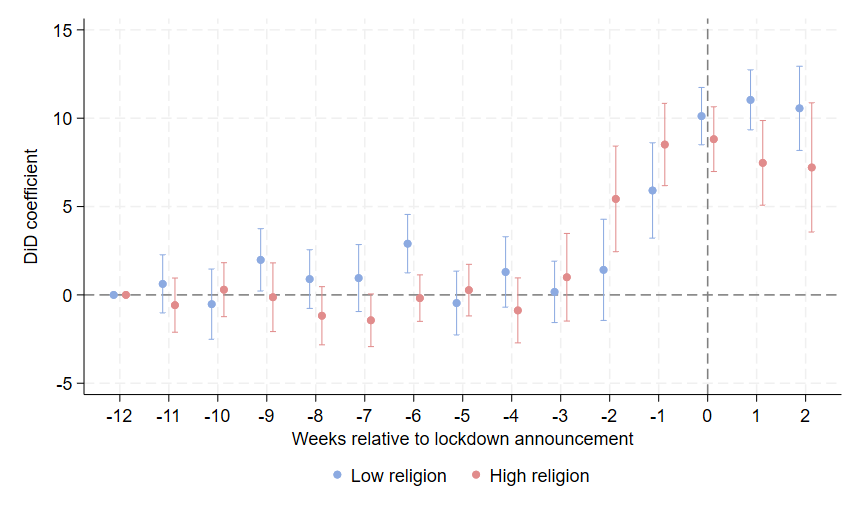
\includegraphics[width=0.75\textwidth]{../Figures/eventstudy_het_God.png} \\
Prayer \\
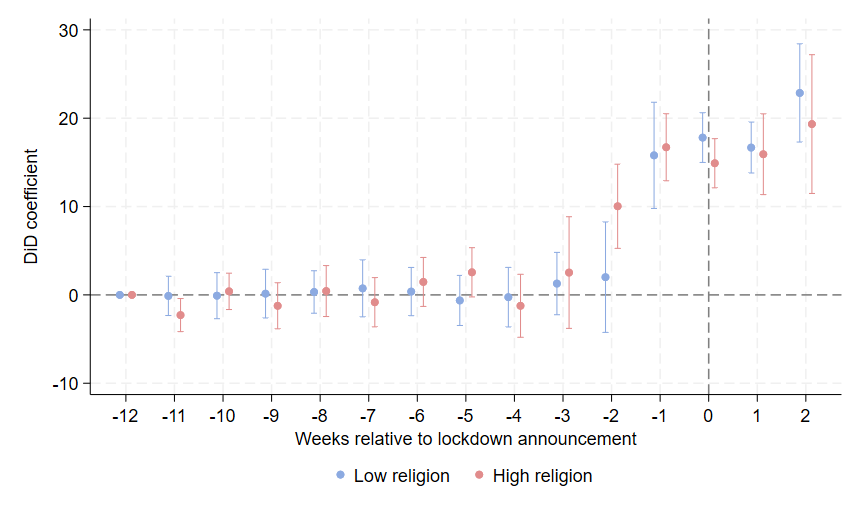
\includegraphics[width=0.75\textwidth]{../Figures/eventstudy_het_Prayer.png} \\
Meditation \\
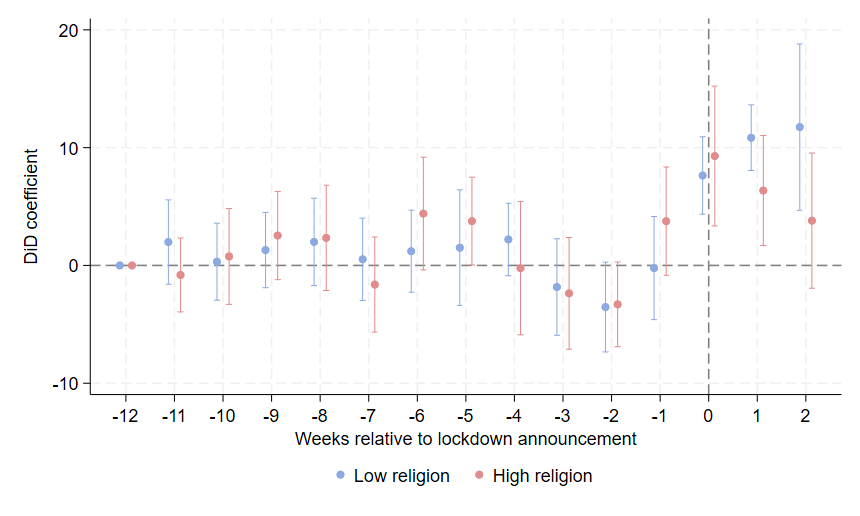
\includegraphics[width=0.75\textwidth]{../Figures/eventstudy_het_Meditation.png} \\
\end{tabular}
\label{fig:eventstudy-het}
\justifying \\ [-3ex]
{\scriptsize \textbf{Notes:} This figure reports event-study coefficients from separate TWFE regressions on low-religion (blue) and high-religion (red) state subsamples. High-religion states are those above the median share of ``very religious'' adults in the Gallup 2017 U.S. Daily tracking survey. Week $-12$ is the omitted reference period. State, year, day-of-year and day-of-week fixed effects included. Confidence intervals at the 95\% level. \par}
\end{figure}

\newpage

%--- TWFE Subcategories ---%
%--------------------------%
\begin{figure}[htbp]
    \centering
    \caption{TWFE estimates on Subcategories}
    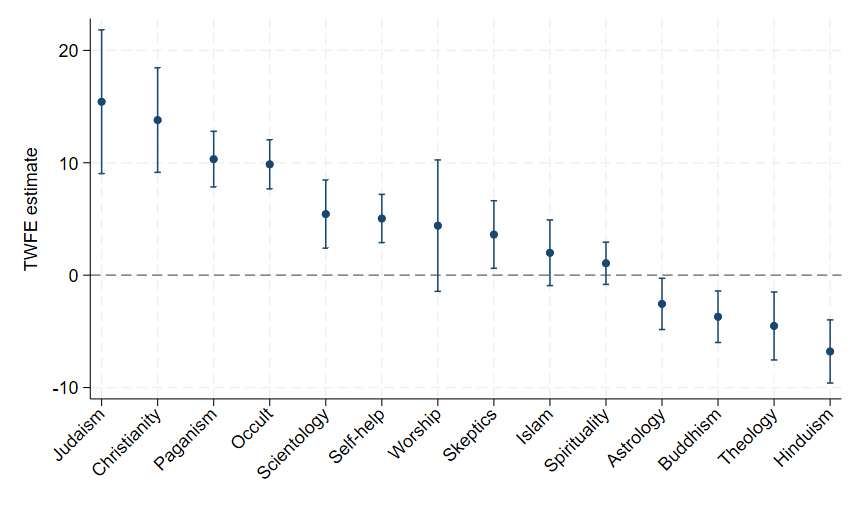
\includegraphics[width=0.9\textwidth]{../Figures/subcat_coef.png}
    \label{fig:subcategories}
\justifying \\ [-1ex]
{\scriptsize \textbf{Notes:} This plots TWFE estimates of each subcategory withing the `Religion \& Belief' category. Confidence intervals at the 95\% level.  \par}
\end{figure}









\end{document}